\documentclass{beamer}
\usepackage{amsmath,amssymb,amsthm,array}
\usepackage{xltxtra}
\usepackage{multirow}
\usepackage{multicol}
\usepackage{algorithm}
\usepackage{hyperref}
\usepackage{algorithmic}
\usetheme{CambridgeUS}
\usecolortheme{crane}
\usefonttheme{serif}
\setmainfont[Mapping=TeX-text]{GFS Neohellenic}
\setbeamertemplate{navigation symbols}{}

\title{Cryptography And Voting}
\author{Panagiotis Grontas}
\date{14/3/2013}
\institute{$\mu \Pi \lambda \forall$}

\setbeamertemplate{footline}
{
  \leavevmode%
  \hbox{%
  
  \begin{beamercolorbox}[wd=1\paperwidth,ht=2.25ex,dp=1ex,right]{title in head/foot}%
    \usebeamerfont{title in head/foot}\insertshorttitle\hspace*{3em}
    \insertframenumber{} / \inserttotalframenumber\hspace*{1ex}
  \end{beamercolorbox}}%
  \vskip0pt%
}
\setbeamerfont{section title}{parent=title}
\setbeamercolor{section title}{parent=titlelike}
\defbeamertemplate*{section page1}{default}[1][]
{
  \centering
    \begin{beamercolorbox}[sep=8pt,center,#1]{section title}
      \usebeamerfont{section title}\insertsection\par
    \end{beamercolorbox}
}
\newcommand*{\addsp}{\usebeamertemplate*{section page1}}

\setlength{\columnseprule}{0.4pt}

\begin{document}

\begin{frame}
\titlepage
\end{frame}

\begin{frame}{Overview}
\begin{itemize}
\item Motivation
\item Cryptography Building Blocks
\item Mixnets: A solution to voter privacy
\item Verifiably Correct Mixnets
\item Almost Verifiably Correct Mixnets
\item Conclusion
\end{itemize}
\end{frame}

\section{Motivation}

\begin{frame}
\addsp
\end{frame}

\begin{frame}{Election Systems: High Level properties}
\begin{itemize}
\item \textbf{Integrity}
\begin{itemize}
	\item Votes are cast as intended
	\item Votes are counted as cast
\end{itemize}
\item \textbf{Ballot Secrecy} Nobody can figure out how you voted (privacy), even if you try to prove it (selling/coercion).
\item \textbf{Authentication and Authorisation}
\begin{itemize}
	\item Only authorised voters can vote
	\item a specified number of times as stated in election law
\end{itemize}
\item \textbf{Enfranchisement} All voters must have the opportunity and be encouraged to vote
\item \textbf{Availability} (Voting,Tallying)
\item \textbf{Efficiency} (Cost,Time)
\end{itemize}
\textbf{Remark: } Authentication vs Secrecy vs Enfranchisement
\end{frame} 

\begin{frame}{Election Systems: Interpretation of properties in building a voting system}
\begin{itemize}
\item \textbf{Privacy} The votes must remain secret
\item \textbf{Individual Verifiability} Each voter can check that their ballot was included in the outcome (\textit{to ensure integrity})
\item \textbf{Universal Verifiability} All voters can check that a voter's ballot was included in the outcome (\textit{to ensure integrity})
\item \textbf{Receipt - Freeness} A voter cannot prove how she voted even if she wants to.
\item \textbf{Robustness} Nobody can disrupt an election (\textit{to ensure availability})
\item \textbf{Fairness} No partial results are known. No vote cancellation/duplication.  (\textit{to ensure availability, integrity, privacy})
\end{itemize}
\textbf{Remark: }Individual Verifiability vs Receipt - Freeness
\end{frame}


\begin{frame}[allowframebreaks]{Electronic Voting For Better Elections(?)}
\begin{itemize}

\item Traditional Systems lack many of the properties we described earlier
\begin{itemize}
\item Lack of Individual/Universal Verifiability (we cast our votes, without verifying that they are counted)
\item Trust is based on tradition and conflict of interest
\end{itemize}

\item By computerising the elections we can actually improve the voting process
\begin{itemize}
\item By counting faster
\item By enabling winner selection by a variety of social choice functions
\item Most importantly: by enabling some of the before mentioned properties
\item We can design the election system, from the ground up following specifications
\end{itemize}

\item But computers themselves introduce many problems 
\begin{itemize}
\item Can we implement systems with conflicting characteristics?
\item Lack Of Transparency
\item eVoting is like voting by proxy. Can we trust another entity to vote for us?
\item For an example: Check the HBO  documentary Hacking Democracy!
\end{itemize}

\framebreak

\item One Solution: Open Source Voting Software
\begin{itemize}
\item Open Source Code can be scrutinised by competing parties and everybody else
\item Voters can build the tallying programs themselves
\item Will surely play a role in the future of voting
\item \textbf{But:} How can we be sure of the actual bits that do the tallying?
\end{itemize}

\item \textbf{The Solution: Cryptography}
\begin{itemize}
\item Cryptography has been used to keep secrets
\item Cryptography can be used to build trust
\item How: By keeping secrecy and providing verification of each operation
\end{itemize}
\end{itemize}
\end{frame}

\section{Cryptography Building Blocks}
\begin{frame}
\addsp
\end{frame}

\begin{frame}{Hash Functions}
A function $h$ that maps arbitrary size data (message) to fixed size data (hash) with the following properties
\begin{itemize}
\item Given the message it is easy to calculate the hash
\item Given the hash it is computationally infeasible to find the message
\item Given a message $m$ it is computationally infeasible to find another message $m'$ such that $h(m)=h(m')$
\item It is computationally infeasible to find two messages $m_1,m_2$ such that $h(m_1)=h(m_2)$
\end{itemize}

\end{frame}

\begin{frame}{Public Key Cryptosystems}
\begin{itemize}
\item Enable exchange of secret messages without prior engagements
\item Introduced by Diffie And Hellman in 1976
\item Each user has a public and a private key
\item In order to send an encrypted message
\begin{itemize}
\item The public key is retrieved
\item The message is encrypted with the it
\item Upon receipt, the message is decrypted with the private key
\end{itemize}
\item Three algorithms are needed (Key Generation, Encryption, Decryption)
\item Security based on (conjectured) hard problems from number theory (factoring, discrete log, quadratic residuosity)
\item Can be turned around to provide signatures (encrypt with the private key)
\end{itemize}
\end{frame}

\begin{frame}[allowframebreaks]{RSA Encryption (1977)}
\begin{itemize}
\item \textbf{Generate keys}
\begin{itemize}
\item  Select Randomly and Independently Two Large Primes $p,q$
\item  Calculate product $n = p \cdot q$
\item  Calculate $ \phi(n) = (p-1) \cdot (q-1)$
\item  Randomly select $ e \in \mathbb{Z}_{n}^{*}$ st: $gcd(e,\phi(n))=1$
\item  Calculate reverse $d = e^{-1} mod \phi(n)$ 
\item  Public key is $(e,n)$ and private key is $(p,q,d)$
\end{itemize}
\item \textbf{Encrypt} Message $m$ : Raise to the public key $c = m^e mod n$
\item \textbf{Decrypt} message $c$ : Raise to the private key $c^d mod n = m^{ed} mod n = m$
\item For security: randomize encryption. Append random padding to the message.
\item if $n$ can be factored than breaking RSA is easy

\item Threshold decryption
\begin{itemize}
\item Break the private key into $n$ pieces so that that $t$ parties can decrypt it
\item Enables the distribution of trust
\end{itemize}

\end{itemize}
\end{frame}

\begin{frame}{Homomorphic Encryption}
\begin{itemize}
\item Computation with encrypted data.
\item $E(m_1) \otimes E(m_2) = E(m1 \oplus m2)$
\item Apply a function to the ciphertexts that corresponds to another function on the plaintexts. The result can be obtained by one decryption.
\item For simple tallying we would require to evaluate a function on ciphertexts that corresponds to adding the plaintexts (additive homomorphism)
\item For other social choice functions we would require computation of arbitrary functions on encrypted data.
\item It can be done ... in theory (Gentry, 2010)
\end{itemize}
\end{frame}

\begin{frame}{ElGamal Encryption (1984)}
\begin{itemize}
\item Randomised Public Key Encryption From Diffie-Hellman Key Exchange
\item Key Generation
\begin{itemize}
\item Select 2 large primes $p,q$ st $q \mid (p-1)$ and a generator $g$
\item Randomly select $ x \in_R \mathbb{Z}_q $
\item Calculate $ y = g^x mod p $
\item Return $ (pk = y, sk = x)$
\end{itemize}
\item Encrypt Message $m$: Multiply with randomisation of public key
\begin{itemize}
\item  Randomly select $r \in_R \mathbb{Z}_q$
\item  Calculate $G = g^r \, mod p$
\item  Calculate $M = m \cdot y^r \, mod p$
\item  Return $ c = (G,M) $
\end{itemize}
\item Decrypt message $(G,M)$ with secret key $x$
\begin{itemize}
\item  return $M/G^x \, mod p$
\end{itemize}
\item Security based on difficulty of computing discrete logs
\end{itemize}
\end{frame}

\begin{frame}[allowframebreaks]{Useful Elgamal properties}
\begin{itemize}
\item \textbf{Reencryption}
\begin{itemize}
\item Change ciphertext without affecting decryption
\begin{align*}
 ReEnc(c,r') & = c \cdot Enc(1,r') = (g^{r+r'},m \cdot (g^x)^{r+r'}) 
\end{align*}
\item No knowledge of secret key is required.
\item Without the secret key or the re randomisation factor it is infeasible to show that two messages are reencryptions of each other.
\end{itemize}
\item \textbf{Multiplicative Homomorphism}
\begin{itemize}
\item Let $m_1, m_2$ plaintexts. Then\textbf{ $Enc(m_1) \cdot Enc(m_2) = Enc(m_1 \cdot m_2)$}
\item In elections we would desire \textbf{additive} homomorphism
\item ElGamal Solution: encrypt message $m$ as $(G,M) = (g^r mod p ,g^m \cdot y mod p)$
\item Problem:Need to solve DLOG, too many exponentiations
\item Other cryptosystems provide additive homomorphism
\end{itemize}
\end{itemize}
\end{frame}

\begin{frame}{Commitments}
\begin{itemize}
\item Commitment Schemes
\begin{itemize}
\item Commit to a value 
\item without revealing it (\textit{hiding} property)
\item and without being able to change it (\textit{binding} property)
\end{itemize}
\item An application: Coin flipping over the telephone
\begin{itemize}
\item Alice and Bob are in different locations but want to flip a coin
\item Alice select head/tails
\item Bob flips the coin 
\item Bob doesn't have to flip the coin, he can just announce that he wins
\begin{block}{Solution}
\item Commit to heads or tails 
\item Flip the coin and announce the result
\item Reveal the commitment
\item Check the result
\end{block}
\end{itemize}
\end{itemize} 
\end{frame}

\begin{frame}[allowframebreaks]{Zero Knowledge Proofs (Goldwasser, Micali, Rackoff - 1985)}
 \begin{itemize}
\item Interactive protocol between 2 parties (prover, verifier)
\item \textbf{Objective:} The prover wants to convince the verifier about the knowledge of a secret, without disclosing (any part) of it
\item Properties:
\begin{itemize}
\item Completeness: Honest prover convinces honest verifier with overwhelming probability
\item Soundness: Dishonest prover cannot succeed with overwhelming probability
\item Zero Knowledge: The verifier cannot learn anything from the protocol
\end{itemize} 
\end{itemize} 

\begin{block}{An illustrating example}
\begin{itemize}
\item \textbf{Prover} holds two \textit{identical} boxes of different color
\item \textbf{Verifier} is color blind
\item \textbf{Prover} wants to convince the Verifier that the boxes have different color
\end{itemize}
\end{block}

\begin{block}{The protocol}
\begin{enumerate}
\item \textbf{Prover} gives the boxes to the verifier
\item \textbf{Verifier} hides the boxes behind her back, one box per hand
\item With probability $\frac{1}{2}$ verifier switches boxes in each hand, behind her back
\item \textbf{Verifier} reveals boxes
\item \textbf{Prover} can tell whether the verifier switched hands
\item Repeat $n$ times to decrease cheating probability to $\frac{1}{2^n}$
\item \textbf{Verifier} is convinced, that the boxes have different color, without ever knowing what it is
\end{enumerate}
\end{block}
\end{frame}

\begin{frame}{Prove that you know DLOG (Schnorr, 1991)}
\begin{center}
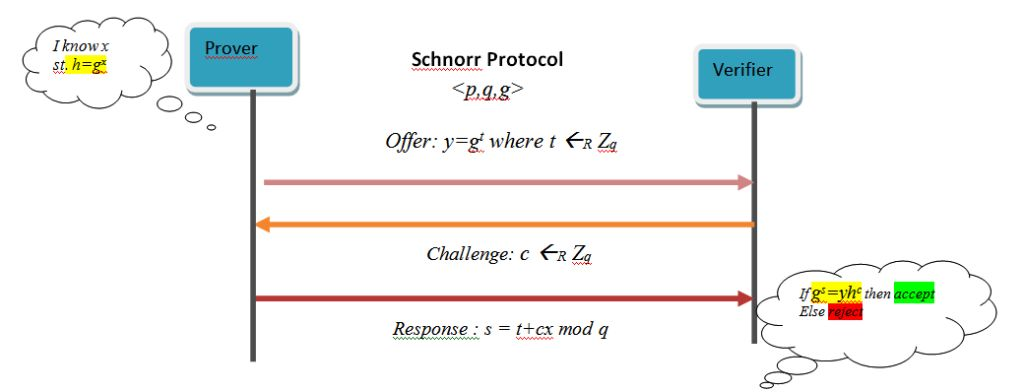
\includegraphics[scale=0.35]{schnorr.jpg}
\end{center}
Authentication using Zero Knowledge Proofs: Prove that you know the password, without revealing it.
\end{frame}

\begin{frame} Prove DLOG equality (Chaum - Pedersen protocol, 1992)
\begin{center}
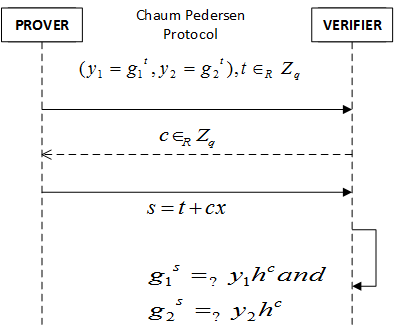
\includegraphics[scale=0.35]{chaumpedersen.jpg}
\end{center}
\textbf{You can Prove Yourself (Fiat - Shamir heuristic, 1987)} Replace verifier with hash function
\end{frame}


\section{Mixnets}

\begin{frame}
\addsp
\end{frame}

\begin{frame}{Overview}
\begin{itemize}
\item A solution to voter privacy - Main idea by David Chaum (1981)
\item Generic primitive for anonymous channel (the original paper has 3500 citations!)
\item Has been used for anonymous email, anonymous browsing, private payment system, multiparty computation and of course \textit{elections})
\item A mixnet consists of a number of mix servers that are operated by different (mistrusting) parties
\item Input: The messages to be anonymised
\item Output: A permutation of the input
\item To achieve anonymity: No single output item, must match an input item
\item An input item is hidden by encryption and shuffling
\item In theory: an honest mix server suffices to achieve privacy
\end{itemize}
\begin{center}

\includegraphics[scale=0.3]{shuffle.jpg}
\end{center}
\end{frame} 

\begin{frame}{Mixnets}
\begin{center}
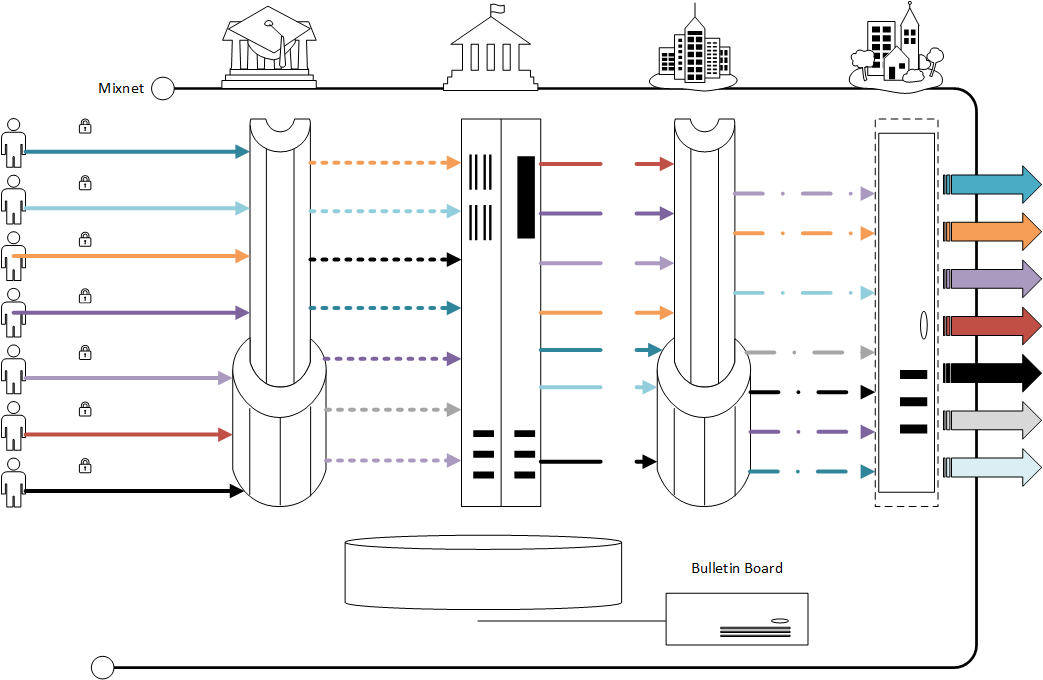
\includegraphics[scale=0.4]{mix.jpg}
\end{center}
\end{frame} 

\begin{frame}{Voting With Mixnets:Main Idea}
\begin{itemize}
\item Voters create their ballots $B_i$
\item Initial Encryption $C_{i0} = Enc(B_i)$
\item Encrypted Ballots enter the mixnet
\item Each mix server permutes and \textit{changes} the encrypted items $C_{\pi_j(i)j} = X_j(C_{ij-1})$
\item After all mixing has occured the \textbf{unencrypted ballots} are posted to the bulletin board
\item The social choice function is computed
\item All communication is achieved by reading from and appending to the bulletin board
\end{itemize}
\end{frame} 

\begin{frame}{Decryption Mixnets}
\begin{itemize}
\item The original Chaum idea
\item Encrypt the ballot with the public key of the mix servers in reverse order
\item $ C_{i0} = E_{pk1} \circ E_{pk2} \circ ... \circ E_{pkt} (B_i) $
\item Each mix server peels of a layer of encryption (decrypts with its secret key) and performs the shuffle
\item After the final stage, all ballots are decrypted
\item \textbf{Remarks:} 
\begin{itemize}
\item Independent of underlying crypto system
\item The ciphertext size is proportional to the number of mix servers
\item A mix server can block the mixing process by refusing to decrypt
\item The last mix server knows the votes and can block the elections (share the final decryption key)
\end{itemize} 
\end{itemize}
\end{frame} 

\begin{frame}{ReEncryption Mixnets - (Park, Itoh, Kurosawa 1993)}
\begin{itemize} 
\item Version 1
\begin{itemize}
	\item Each mix server re randomises the ballots by reencryption
	\item A final decryption stage is needed
	\item The decryption key must be shared to various parties
	\item The decryption is jointly done by all mix servers.
\end{itemize}
\item Version 2
\begin{itemize}
	\item Combines decryption and reencryption
	\item Each mix server partially decrypts the ballots by applying its secret key.
	\item Then re randomises by reencryption
	\item The last mix server decrypts
\end{itemize}
\end{itemize}
\end{frame} 

\begin{frame}[allowframebreaks]{A basic attack (Pfitzmann, 1995)}
Active Attack: Trace an encrypted input by injecting a correlated message
\begin{block}{Track input $m_i$ for participant $P_i$}
\begin{itemize}
\item Initial Encryption $c_{i0} = (g^R, m_i \cdot (y_1,\cdots,y_k)^R)$
\item Mix server j input: $c_{ij} = (g^{R'}, m_i \cdot (y_j,\cdots,y_k)^{R'}) = (t,u)$
\item For some random $x$ generate $c^{''}_{ij} = (t^x,u^x)=(g^{R'x}, m_{i}^{x} \cdot (y_j,\cdots,y_k)^{R'x})$
\item Output will contain both $m_{i}^{x},m_{i}$
\item Raise all output messages to the $x$ and check for duplicates.
\end{itemize}
\textit{Reminder: } El Gamal has multiplicative homomorphism ($E(m)^x = E(m^x)$)
\end{block}

\begin{block}{Track input $m_1, ..., m_s$ for participants $P_i, ..., P_s$}
\begin{itemize}
\item Choose random values $x_1, ..., x_s$
\item Calculate $c = \prod_{i=1}^{s} c_{ij}^{x_i}$
\item Inject or replace with $c$
\item Output will contain the decryption $m*$ of $c$ 
\item Look for s messages such that $m* =  \prod_{i=1}^{s} m_i^{x_i}$
\end{itemize}
\end{block}

\begin{block}{Remarks}
\begin{itemize}
\item Applies to both decryption and reencryption mixnets
\item If there is a check on number of input items a colluding participant's message must be omitted
\item Solution: Redundancy in messages in order to detect the attack
\begin{itemize}
\item Increases Ciphertext Size
\item Does not work if the last mix server is corrupt, since it can replace the $m_{i}^{x}$ with a correct looking message after the message correlation
\end{itemize} 
\item Something stronger is needed
\end{itemize}
\end{block}
\end{frame}


\begin{frame}{Problems}
\begin{block}{Problems}
\begin{itemize}
\item At the initial encryption stage, a different vote might be encrypted (vote changing, vote copying, vote cancelling)
\item A mix server can change some of the input votes, by replacing them in the output.
\item A subset of the mix servers might cooperate to break anonymity by tracing messages
\end{itemize}
\end{block}

\begin{center}
\begin{large}
Solutions must be efficient, correct and privacy respecting
\end{large}
\end{center}

\end{frame} 

\begin{frame}{Solutions}
\begin{block}{Main Idea}
\begin{itemize}
\item Zero - knowledge proof of the contents of the vote
\item Zero - knowledge proof of the correctness of the shuffle
\end{itemize}
\end{block}

\begin{itemize}
\item Correctness of initial encryption $ \Leftrightarrow $ Prove that you know DLOG
\item Correctness of Shuffling   $ \Leftrightarrow $ \\
 	 Prove that each encrypted vote in the input, appears in the output  in a valid reencrypted form
\end{itemize}
\end{frame}

\section{Verifiable Mixnets}
\begin{frame}
\addsp
\end{frame}

\begin{frame}[allowframebreaks]{Killian-Sako Verifiable Mixnet (1995)}
\begin{itemize}
\item The first universally verifiable mixnet
\item Elgamal Reencryption based Mixnet 
\item Verification based on cut and choose protocol
\end{itemize}
\begin{block}{Cut - And - Choose Proof Of Correct Reencryption}
\begin{itemize}
\item Prove knowledge of secret key and partial decryption.
\item Perform secondary reencryption with new randomisation factor
\item Reveal secondary reencryption or difference between primary and secondary reencryption
\end{itemize}
\end{block}

\begin{block}{Cut - And - Choose Proof Of Correct Shuffle - Main idea}
\begin{itemize}
\item Each mix server generates another permutation and randomisation values
\item Perform reencryption and shuffling according to them (secondary shuffle)
\item Reveal secondary shuffle or the difference between primary and secondary shuffle
\end{itemize}
\end{block}
\end{frame}


\begin{frame}[allowframebreaks]{Mixnets based on permutation networks - 1999}
\begin{itemize}
\item Each mix server $M_i$ simulates a sorting network.
\item Reencrypts then sorts the inputs
\item The mix server is built in a bottom up  by combining smaller comparator functions
\item \textbf{Proof Of Correctness:} Prove for a $2 \times 2$  sorting network using the Chaum-Pedersen Protocol 4 times and generalise for $n \times n$ sorting network
\end{itemize}
\begin{center}
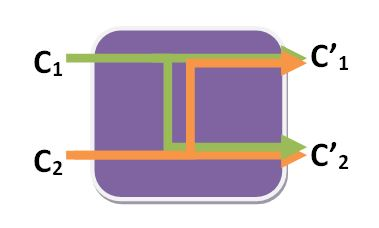
\includegraphics[scale=0.3]{Mix2x2.jpg}
\end{center}


\end{frame}

\begin{frame}[allowframebreaks]{Furukawa and Sako Mixing - 2001}
\begin{itemize}
\item Mixing is represented as matrix multiplication.
\item Permutation matrix
\[
A_{ij} = \begin{cases} 1, \pi(i)=j \\ 0, \text{otherwise} \end{cases}
\]
\item For example the permutation $\pi(1,2,3) = (2,3,1)$ can be represented using the matrix:
\[\begin{bmatrix}
  0 & 1 & 0 \\
  0 & 0 & 1 \\
  1 & 0 & 0
 \end{bmatrix}\]
\item Shuffling and re encryption can be represented using a permutation matrix.
\item Prove that $r_i$ and $[A_{ij}]$ exists based on the key observation that a matrix $[A_{ij}]$ is a permutation matrix iff the dot product of two columns is 0 (if they are different) and 1 (if they are the same)
\end{itemize}
\end{frame}

\begin{frame}[allowframebreaks]{Neff Verifiable Mixnet (2001, 2003)}
\begin{itemize}
\item Mix inputs and outputs are represented as polynomials $P_{in}, P_{out}$
\item Key Property: A polynomial is unaffected by permutation of the roots.
$ \prod_{i=1}^n (m_i - x) = \prod_{i=1}^n (m_{\pi(i)} - x) $
\item Verifier chooses a random $t \in Z_q$
\item Evaluates both input and output polynomials
\item The results match with very high probability
\end{itemize}
\end{frame}

\begin{frame}{Verifiable Mixnets: Performance}
Cost = Total Number of Exponentiations For
\begin{itemize}
\item Initial Encryption
\item Proof of Reencryption and Shuffling
\item Decryption
\end{itemize}
Performance for $n$ voters and $k$ mix servers:
\begin{itemize}
\item \textbf{Sako - Killian} $642nk$
\item \textbf{Sorting Networks}  $7nlogn(2k-1)$
\item \textbf{Furukawa Sako} $18n(2k-1)$
\item \textbf{Neff} $8n(2k-1)$
\end{itemize}
In practice: Neff Mixnet: $10^6$ votes $ \Rightarrow 20$ hours to mix and verify. \\
\begin{center}
\textbf{Lesson}:Zero Knowledge Proofs Are Computationally Expensive.
\end{center}
\end{frame}

\section{Almost Verifiable Mixnets}
\begin{frame}
\addsp
\end{frame}

\begin{frame}[allowframebreaks]{Randomised Partial Checking}

\begin{itemize}
\item RPC - Jakobsson, Juels, Rivest - 2001
\item Create an efficient verifiable mixnet out of any cryptosystem
\item \textbf{Idea}: Give up the expensive notion of \textbf{proof}
\item Provide \textbf{strong evidence} that the mix server has operated correctly (ie. the output is a processed permutation of the input)
\item Strong Evidence = Probabilistic Verification
\item Partial Revelation of the input/output correspondence.
\item For $n$ items, choose randomly $\frac{n}{2}$ and reveal the input/output relation.
\item The mix server has no control of which items are revealed.
\item \textbf{Objective:} A cheater cannot get away with altering too many votes
\item \textbf{Tradeoff:} Privacy and Correctness
\end{itemize}

\begin{block}{Operation}
\begin{itemize}
\item $X_j$ is a cryptographic operation that transforms ciphertext $c$ to $c'$ (reencryption, decryption)
\item Mix server $M_j$ randomly selects a permutation $\pi_j$
\item Commit to the permutation by publishing to the bulletin board
\begin{itemize}
\item A commitment $\Gamma_j^{in}$ that input i maps to output $\pi_j(i)$, if $j$ is odd
\item A commitment $\Gamma_j^{out}$ that output i came from $\pi^{-1}_j(i)$, if $j$ is even
\end{itemize}
\item Proof of correct operation: \textbf{Partial} Revelation
\begin{itemize}
\item  Reveal information that allows anyone to verify that $c_{ij}=X_j(c_{kj-1})$
\item  What to reveal: randomness, $i$, $k$
\item  Also reveal the commitments
\end{itemize}
\item Verifier validates the transformation
\end{itemize}
\end{block}

\begin{block}{What about privacy}
\begin{itemize}
\item Main idea:Pair the servers so that we never reveal the same correspondence twice.
\item Only the inter-pair correspondences are revealed
\item Let $j$ odd and $(M_j,M_{j+1}) \text{ a server pair }$. Then
\begin{itemize}
\item $P_{IN}(Q_j,k)=false$
\item $P_{OUT}(Q_j,i)=true \text{ with probability } \frac{1}{2}$
\item $P_{IN}(Q_{j+1},i)=1-P_{OUT}(Q_j,i)$
\item $P_{IN}(Q_{j+1},m)=false$
\end{itemize}
\item At least one honest pair is needed for privacy
\end{itemize}
\end{block}

\begin{center}
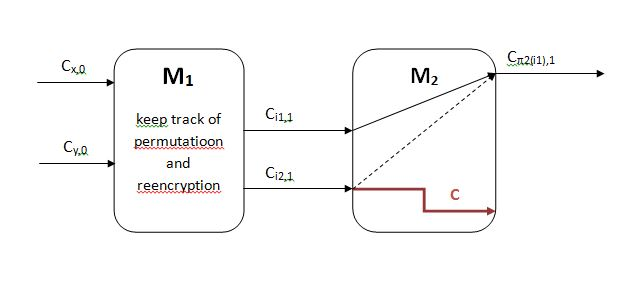
\includegraphics[scale=0.5]{rpc.jpg}
\end{center}


\end{frame}

\begin{frame}[allowframebreaks]{Almost Entirely Correct Mixing (Boneh, Golle - 2002)}

\begin{itemize}
\item \textbf{Idea}: Sacrifice the validation of correctness for speed.
\item An almost correct proof of mixing might suffice, if the margin of victory is high
\end{itemize}

\begin{block}{Method}
\begin{itemize}
\item Select a random subset $S$ of mix server inputs
\item Calculate the product $\pi_s$
\item Reveal $S$ to the mix server.
\item Ask to product a set of outputs $S'$ st. $\pi_s = \pi_{s'}$
\item Honest mix server:  Simply apply the permutation
\item Cheating mix server: \textbf{Might} be impossible to find such $S'$.
\end{itemize}
\end{block}


\end{frame}

\begin{frame}[allowframebreaks]{Optimistic Mixing (Golle, Zhong, Boneh, Jakobsson, Juels - 2002)}

\begin{itemize}
\item Concept based on almost entirely correct mixing
\item Fast proof when all mix servers are honest
\item Reminder: Product preservation might not imply absence of cheating
\item Cheating might be discovered, albeit after the fact. Privacy would be exposed.
\item Solution: Augment with cryptographic checksums and check both product and checksums
\item If a cheating mix server is found then:
\begin{itemize}
	\item No output is produced
	\item A correct proof is executed (Neff, Furukawa-Sako)
	\item Privacy is not compromised
\end{itemize}
\item \textbf{Details:}User input is encrypted twice!
\begin{itemize}
\item Encrypt the vote
\item Hash the encryption components
\item Encrypt the hash.
\end{itemize}
\item Mixing proceeds as usual with permutation and reencryption
\item Verification: Decrypt once and check products and checksums
\item If verification succeeds then everything is OK. Decrypt the vote and tally.
\item If cheating is discovered then the cause of cheating is sought for the triples that do not checksum.
\item How: 
\begin{itemize}
\item Starting from the end each server reveals  (input, randomisation) for the triples in question.
\item If the first server is reached than the mix worked correctly.
\item Cheating was due to the users. Solution: Ignore the cheating senders and count the vote.
\item If a server is exposed as cheating then repeat with slower and verifiable mixnet.
\end{itemize}
\item Cheating will not expose privacy, since the cheating server will occur on (single) ciphertexts
\end{itemize} 
\end{frame}

\section{Conclusion}
\begin{frame}
\addsp
\end{frame}

\begin{frame}{Conclusion}
\begin{itemize}
\item Electronic voting \textbf{can} improve the voting process 
\item If implemented correctly, it allows for properties that are not found even in the traditional systems that we have grown to trust
\item Cryptography can help rebuild that trust, by allowing for secrecy and verification 
\item Mixnets are a mature technology that has been extensively researched in the last 20 years and can be used to anonymise the votes
\item There exist many protocols for mixnets that combine efficiency, correctness, privacy to some extent
\item Many eVoting systems rely on mixnets (Pret A' Voter, Verificatum)
\item The building blocks are there but much work must be done in their composition, implementation and proof of security
\item The goal however remains: 'Trust nothing but verify everything' (\textit{Ben Adida - creator of Helios})
\end{itemize}

\begin{center}
\begin{Huge}
Thank you!
\end{Huge}
\end{center}

\end{frame}

\section{References}
\begin{frame}
\addsp
\end{frame}

\begin{frame}[allowframebreaks]{References}
\begin{tiny}
\bibliographystyle{alpha}
\bibliography{refs}
\end{tiny}
\nocite{*}
\end{frame}

 
\end{document}
